\subsection{Duality: Two-sided Tests and Two-sided Confidence Intervals}
\label{subsec:duality}

An interesting fact can be discovered if we look into our derivation of tests and confidence intervals. It turns out that we can conduct two-sided tests using nothing but the confidence intervals!
\begin{formula}{(Eq. 21)}
  A level $\alpha$ Z-test of $H_0\ :\ \theta = \theta_0$ vs $H_A\ :\ \theta \neq \theta_0$ accepts the null hypothesis 
  
  \begin{center}\textit{\textbf{if and only if}}\end{center}

  a symmetric $(1 - \alpha)100\%$ confidence Z-interval for $\theta$ contains $\theta_0$.
\end{formula}
\setcounter{equation}{21}

\begin{figure}[H]
  \centering
  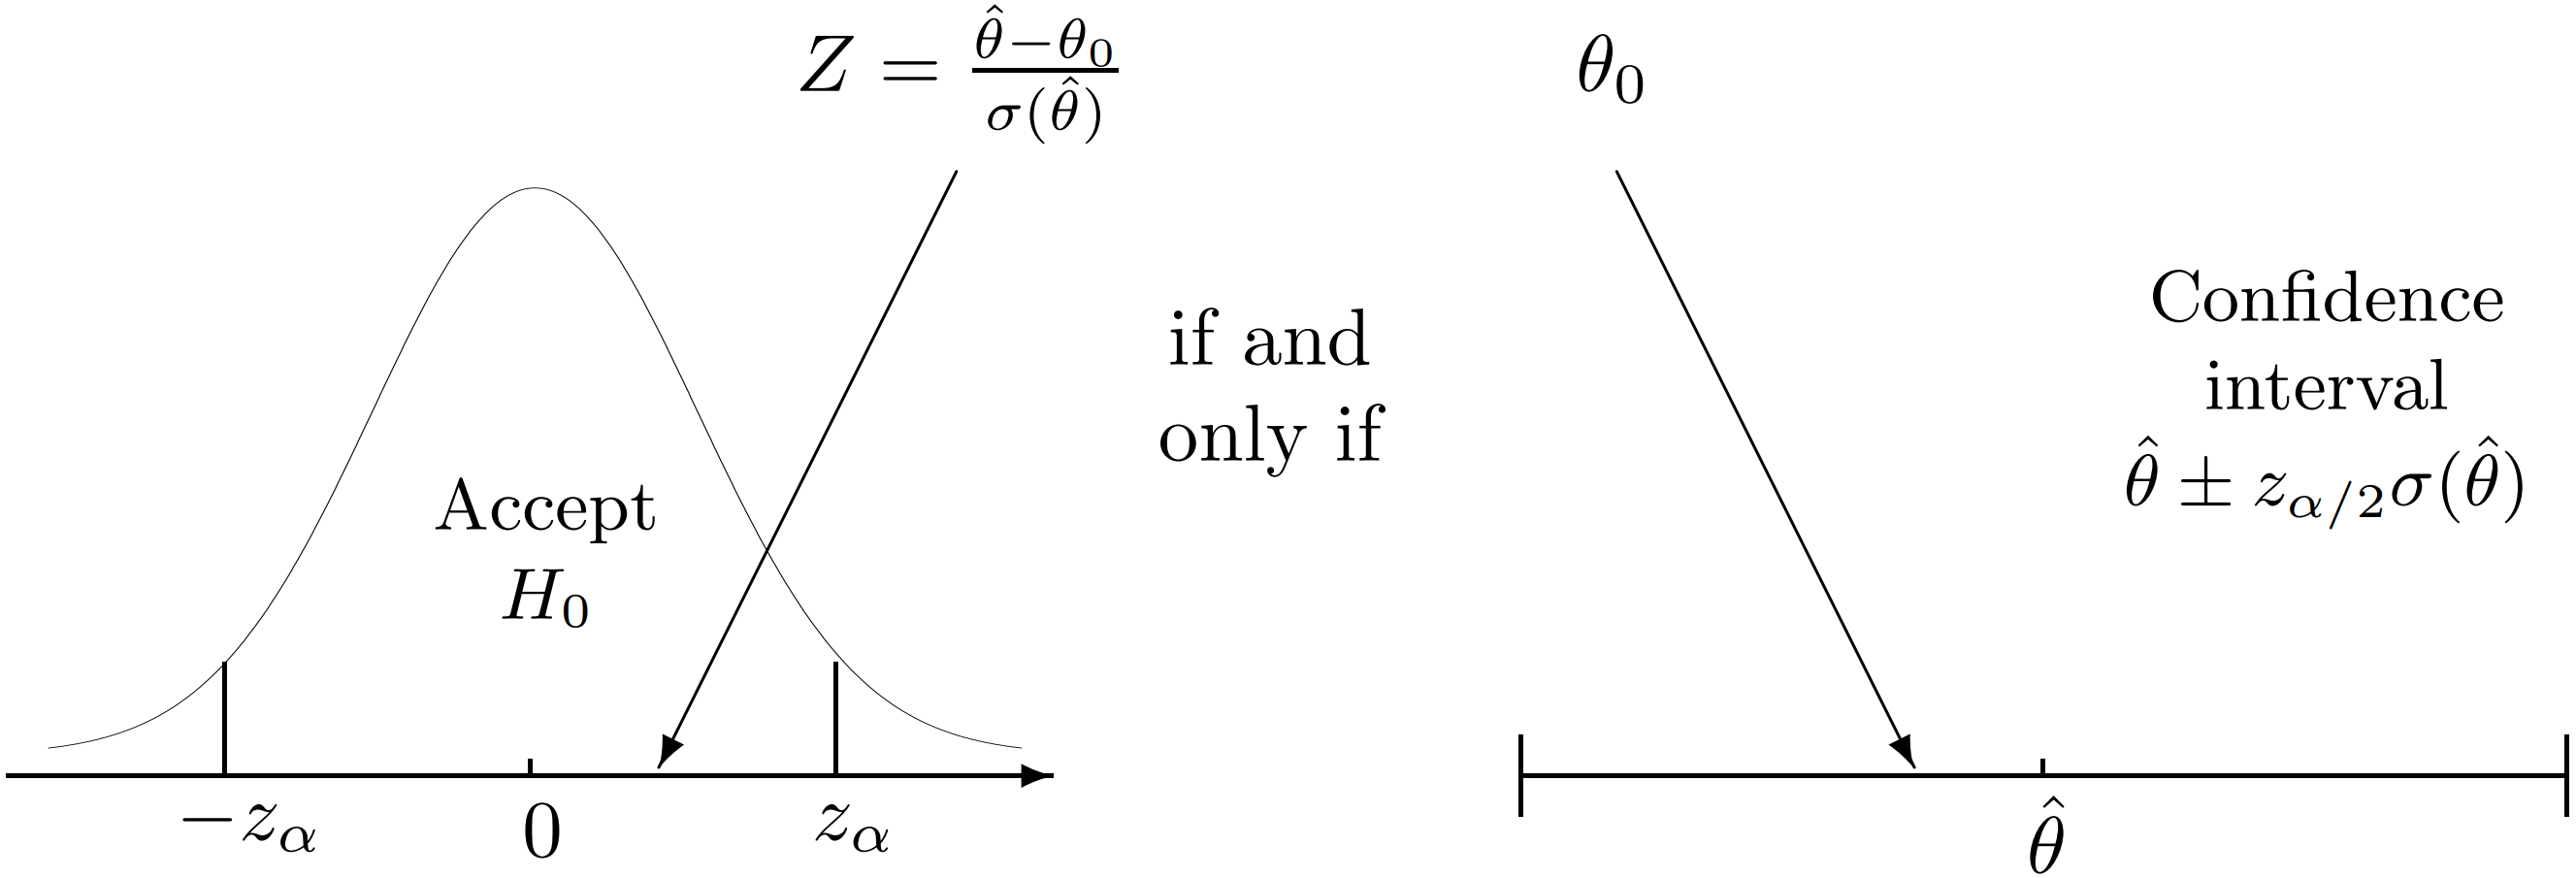
\includegraphics[width=\linewidth]{img/fig-9.8.png}
  \caption{}
\end{figure}

In fact, any two-sided test can be conducted this way. Accept $H_0\ :\ \theta = \theta_0$ whenever a $(1 - \alpha)100\%$ confidence interval for $\theta$ covers $\theta_0$. Under $\theta_0$, this test will accept the null
hypothesis as often as the interval will cover $\theta_0$, i.e., with probability $(1 - \alpha)$. Thus, we have a level $\alpha$ test.

Rule (21) applies only when
\begin{itemize}
  \item we are testing against a two-sided alternative (notice that our confidence intervals are two-sided too);
  \item significance level $\alpha$ of the test matches confidence level $(1 - \alpha)$ of the confidence interval. For example, a two-sided $3\%$ level test can be conducted using a $97\%$ confidence interval.
\end{itemize}

\begin{example}{}
  A sample of 6 measurements
  \begin{center}
    2.5, 7.4, 8.0, 4.5, 7.4, 9.2
  \end{center}
  is collected from a Normal distribution with mean $\mu$ and standard deviation $\sigma = 2.2$. Test whether $\mu = 6$ against a two-sided alternative $H_A\ :\ \mu \neq 6$ at the $5\%$ level of significance.

  \textbf{Solution:}
  Solving Example 4, we have already constructed a $95\%$ confidence interval for $\mu$,
  \begin{equation*}
    \left[ 4.74,\ 8.26 \right]
  \end{equation*}
  The value of $\mu_0 = 6$ belongs to it; therefore, at the $5\%$ level, the null hypothesis is accepted.
\end{example}

\begin{example}{}
  Use data in Example 13 to test whether $\mu = 7$.

  \textbf{Solution:}
  The interval $\left[ 4.74,\ 8.26 \right]$ contains $\mu_0 = 7$ too; therefore, the hypothesis $H_0\ :\ \mu = 7$ is accepted as well.
\end{example}

\textbf{\textit{Check examples 9.33, 9.34, 9.35 in the textbook}}.

Similarly, for the case of unknown variance(s).
\begin{formula}{}
  A level $\alpha$ T-test of $H_0\ :\ \theta = \theta_0$ vs $H_A\ :\ \theta \neq \theta_0$ accepts the null hypothesis 
  
  \begin{center}\textit{\textbf{if and only if}}\end{center}

  a symmetric $(1 - \alpha)100\%$ confidence T-interval for $\theta$ contains $\theta_0$.
\end{formula}
